\subsection{Dealing with 1-player Battleship Problem Using GBSC}
Recall the 1-player Battleship problem:
$$    \min_{Q_1, Q_2, \dots, Q_T} T  , Q_t = (i_t, j_t)$$
$$    \mathcal{X}_t = \{X|(X\in \mathcal{X}_{t-1}) \wedge (X_{i_t j_t} = X^{*}_{i_t j_t})\} , 1 \leq t \leq T$$
$$\mathcal{X}_0 = \{ X_1, X_2, X_3, \dots, X_n \},	\mathcal{X}_T = \{X^{*}\}, \text{ random variable } X^* \in \mathcal{X}_0 $$

$\mathcal{X}_0$ is a set of $0-1$ matrices representing the entire possible board space without any prior knowledge, and $X^*$ is the target board chosen by the opponent (randomly sampled from $\mathcal{X}_0$ in our case).

More precisely, we would like to minimize the average number of tries $T$ over all possible targets $X$.

By assumption, the target board $X^{*}$ is randomly sampled from $\mathcal{X}_0$. The key to minimizing the number of queries $t$ is to choose the queries $Q_1, Q_2, \dots, Q_T$ such that the size of remaining possible boards, $|\mathcal X_{t}|$ converges to $1$ quickly. 

Using the conclusions from GBSC coding, we can devise a way to minimize the average number of queries.
At $t$-th query, the hit probability matrix is 
$$P^{(t)}_{ij} = \frac{\sum_{X \in \mathcal{X}_{t-1}} X_{ij}}{|\mathcal{X}_{t-1}|}   $$

Obviously, the hit probability of some previously queried $(i,j)$ is either $0$-missed or $1$-hit. So there is no need to query the same grid twice.

we choose $Q_t$ by this greedy strategy, deducted from GBSC:
$$Q^*_t=(i^*_t, j^*_t) = \arg\min_{(i,j)} |P^{(t)}_{ij} - \frac{1}{2}| $$.

Ideally, each query $(i^*_t, j^*_t)$ will half the size of the remaining boards space, giving us the average number of queries $\bar{T} = \lceil \log n \rceil$, where $n = |\mathcal{X}_0|$. Of course, this is not always possible in the real world, since there may not be exist a $(i,j)$ with $p^t_{ij} = \frac{1}{2}$. Nonetheless, we can always choose the grid with hit probability closest to $\frac{1}{2}$ and get a sub-optimal algorithm.

\begin{algorithm}[H]
	\caption{Solving 1-player Battleship using GBSC.} 
	\begin{algorithmic}[1]
    \State calculate initial possible board space $\mathcal{X}_0$
    \State $t \gets 0$
    \While{$|\mathcal{X}_t| > 1$}
        \State $t \gets t + 1$
        \State $P^{(t)}_{ij} \gets \frac{\sum_{X \in \mathcal{X}_{t-1}} X_{ij}}{|\mathcal{X}_{t-1}|}   $
        \Comment{calculate hit probability matrix}
        % \State $Q^*_t=(i^*_t, j^*_t) = \arg\min_{(i,j)} |P^t_{ij} - \frac{1}{2}| $ // Choose locally optimal query 
        \State $Q^*_t \gets \arg\min_{(i,j)} |P^t_{ij} - \frac{1}{2}| $ 
        \Comment{choose locally optimal query}
        \State $\mathcal{X}_t \gets \{X|(X\in \mathcal{X}_{t-1}) \land (X_{i^*j^*} = X^{*}_{i^*j^*})\}$
        %\Comment{eliminate some boards in $\mathcal{X}_{t-1}$ and get $\mathcal{X}_t$} 
        \Comment{eliminate some boards in $\mathcal{X}_{t-1}$} 
    \EndWhile
    \State $\mathcal{X}_t = \{X^*\}$
	\end{algorithmic} 
	
\end{algorithm}

% Later we will demonstrate the effectiveness of this algorithm by playing simulated games of Battleship.

%----------------------------------------------------------------------------------------
% Analysis
%----------------------------------------------------------------------------------------

% \section{Results} \label{Results}
% \subsection{GBSC: 1-player Battleship}

We did some tests to show the effectiveness of the GBSC-based algorithm on dealing with 1-player Battleship problem. To speed up computation, we consider 3 ships of length 5, 4 and 3 placed on a $10\times 10$ board. In total, there are $n=\num{1850736}$ possible board layouts, which is just under $2^{21}$. Here we define the number of tries $t$ as the number of queries to determine the target board $X^*$.\footnote{Sometimes two or more boards may be different yet indistinguishable, and the terminal entropy is nonzero, for example if two boats of length 3 and 4 are adjacent and from a L-shape pattern. Since this does not affect the outcomes, we consider these boards to be identical.}Since each query (bombing) in average gives at most $1$ bit of information,  the theoretical minimal average number of tries is $\bar{T}^* = \lceil \log n \rceil  = 21$ queries. Of course, one can sometimes get lucky and determine $X^*$ in less than $21$ tries.



Here we have 10 randomly chosen target boards for our algorithm to play against. The vertical axis is calculated by $H(X) = \log |\mathcal{X}_t|$. Again, we assume that every target board has the same probability of being chosen.
\begin{figure}[H]
    \centering
    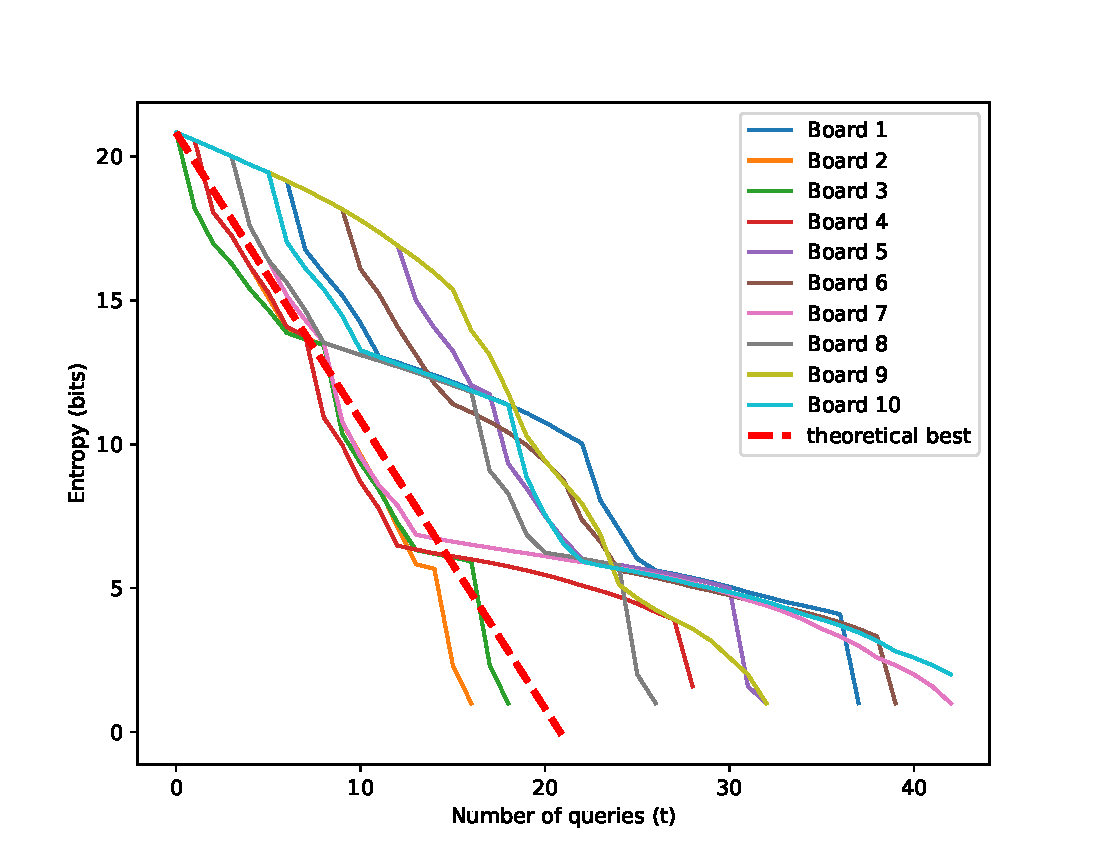
\includegraphics[width=0.5\textwidth]{figure/battleship_10_1.pdf}
    \caption{Algorithm against 10 random boards v.s. theoretical best average}
    \label{fig:Battleship10}
\end{figure}



We can observe two types of stages in the declination of entropy: at first, the entropy declination is usually slow, as the algorithm knows very little about the board and is exploring the board. When a "hit" occurs, the entropy drops rapidly, before the information provided by this hit is fully exploited, and this process repeats until entropy drops to 0. 



For this small scale test, the results are very diverged. Some were very lucky and better than the theoretical best average $21$, and some are almost 2 times of theoretical best average. We ran the same test on a larger scale, on 1000 randomly chosen target boards and got some interesting results.

\begin{figure}[htb]
    \centering
    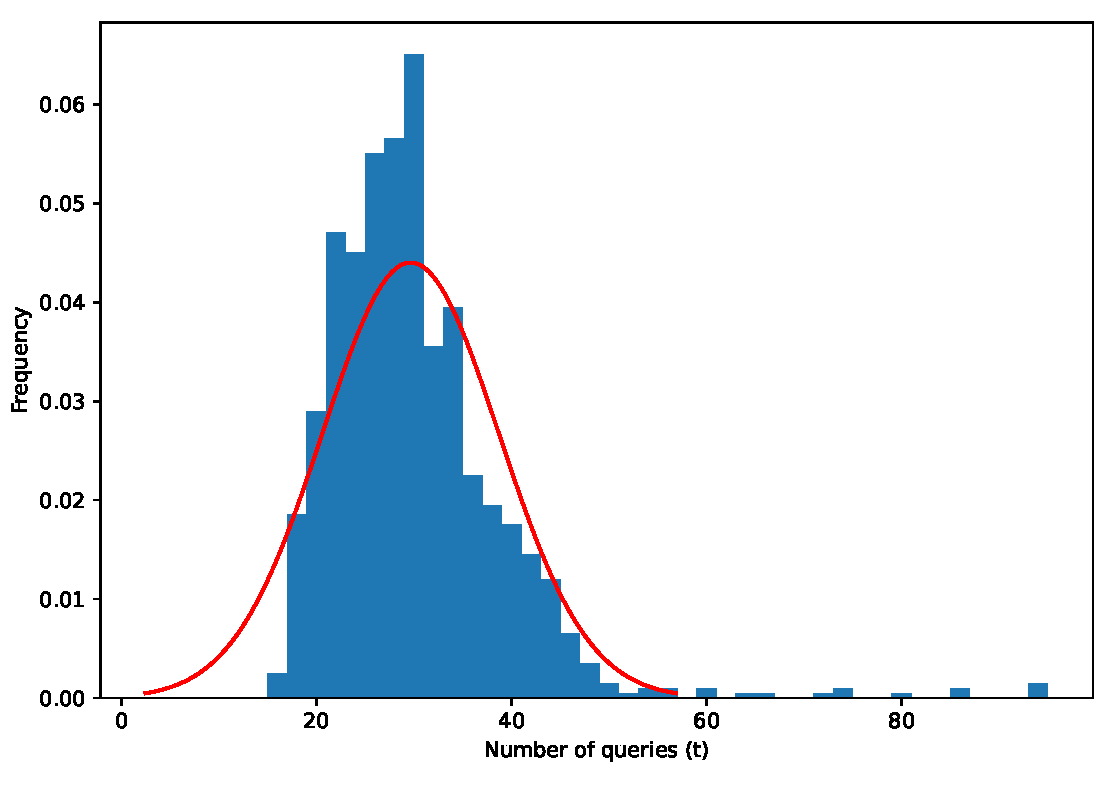
\includegraphics[width=0.5\textwidth]{figure/1000_hist.pdf}
    \caption{Distribution of queries to determine target board $X^*$}
    \label{fig:Hist1000}
\end{figure}
The mean number of queries $\bar{T}= 29.651$ and the standard deviation $\sigma =  9.062$. From this we can conclude that our GBSC-based algorithm performs reasonably well for Battleship, since $\bar{T}\approx 1.4 \bar{T}^*$. We can also take a look at the actual strategy of our algorithm for one game. This visualization (Fig.\ref{fig:Pmatrix}) shows how the algorithm prefers hit probability closest to 0.5.
\begin{figure}
    \centering
    \begin{subfigure}{0.35\textwidth}
        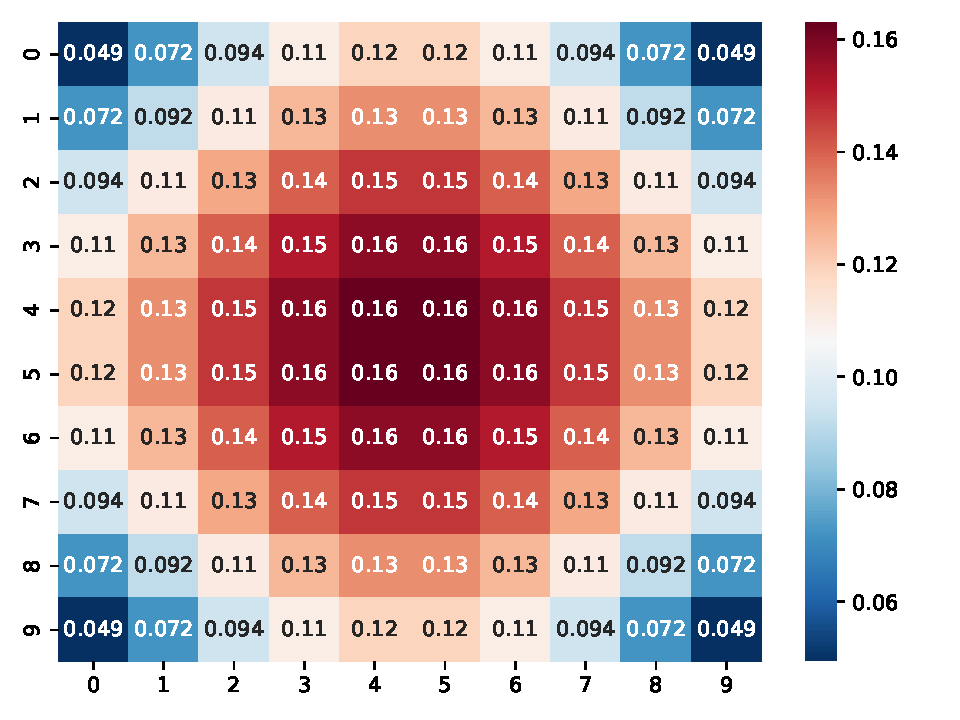
\includegraphics[scale=0.4]{figure/pmatrix/0.pdf}
        \caption{t=0}
    \end{subfigure}
    \begin{subfigure}{0.35\textwidth}
        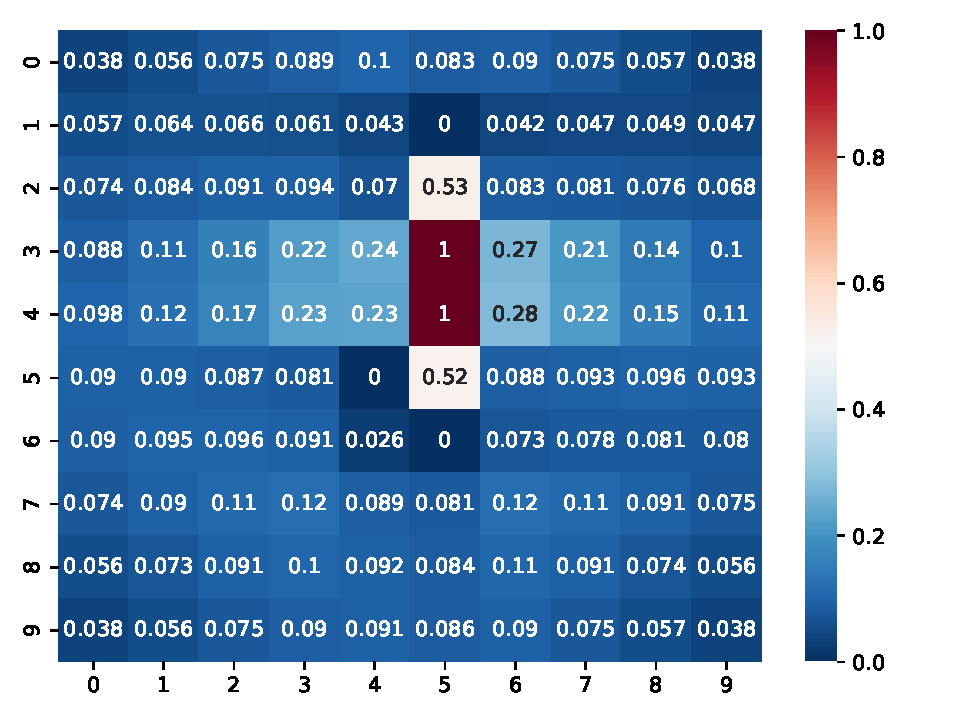
\includegraphics[scale=0.4]{figure/pmatrix/5.pdf}
        \caption{t=5}
    \end{subfigure}
    
    
    \begin{subfigure}{0.35\textwidth}
        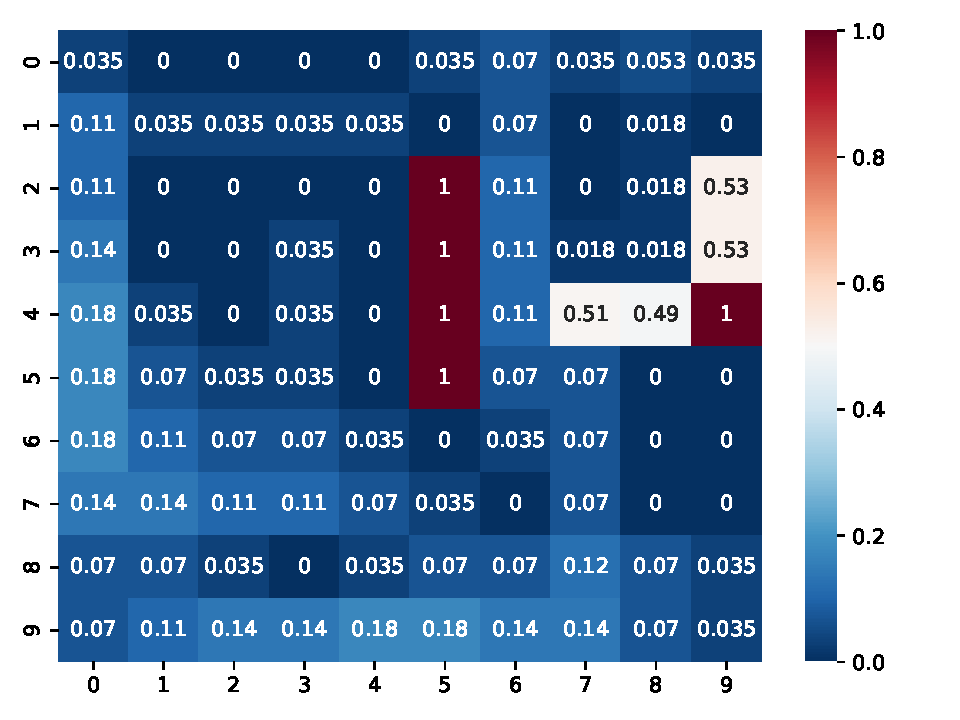
\includegraphics[scale=0.4]{figure/pmatrix/19.pdf}
        \caption{t=19}
    \end{subfigure}
    \begin{subfigure}{0.35\textwidth}
        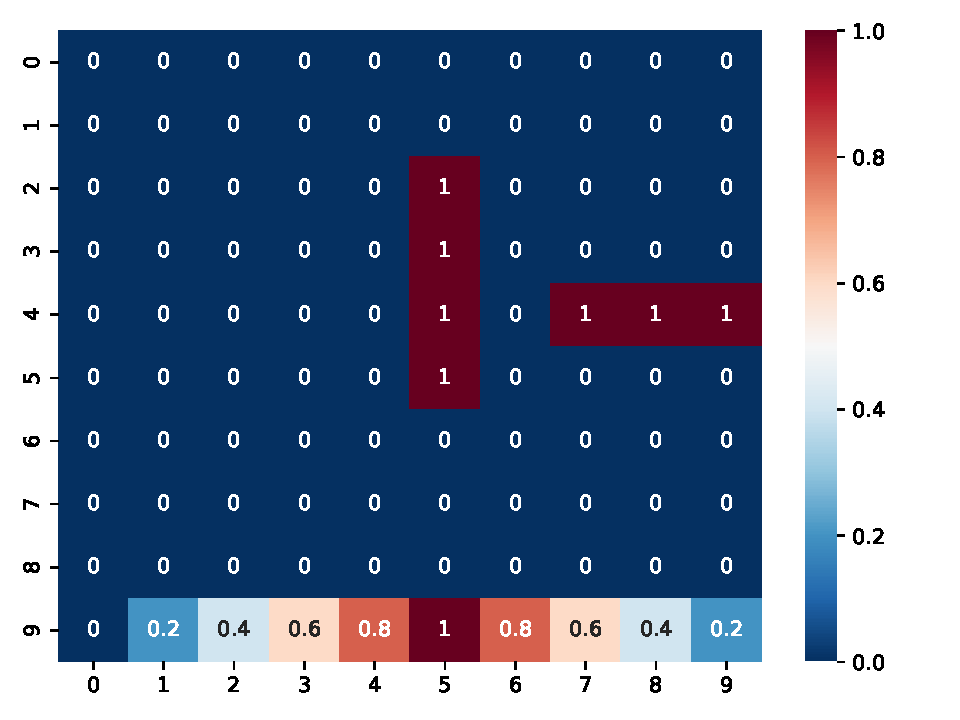
\includegraphics[scale=0.4]{figure/pmatrix/22.pdf}
        \caption{t=22}
    \end{subfigure}
    \caption{Hit probability matrix visualized. $p_{ij}:$ 0=No ship, 1=Has ship, (0,1)=Uncertain}
    \label{fig:Pmatrix}
\end{figure}

In another game, we demonstrate the hit pattern of our algorithm. (Fig.\ref{fig:Hitpattern}) Interestingly, our algorithm displays a diagonal search strategy, which is not intentionally designed in our GBSC based algorithm, but rather the result of computing the hit probability matrix, because a miss at $(i,j)$ reduces the conditional probability at $(i+1,j), (i-1,j),(i,j+1),(i,j-1)$. Also notice that the diagonal bombing lines are 3 grids apart, making a 4-long ship impossible to fit in the center area. Therefore, a diagonal searching pattern is great for quickly reducing entropy. This increases our confidence about this GBSC-based algorithm, since trying to hit the ships by bombing a diagonal pattern is a well-known strategy in this classic game, which also coincides with some previous deterministic approaches\cite{Rodin}.

\begin{figure}[H]
    \begin{center}
    \begin{subfigure}{0.2\textwidth}
    \begin{tikzpicture}
    \matrix[boardstyle]{
        |[w]|& |[w]|& |[w]|& |[w]|& |[w]|& |[w]|& |[w]|& |[w]|& |[w]|& |[w]|\\
        |[w]|& |[w]|& |[w]|& |[w]|& |[w]|& |[w]|& |[w]|& |[w]|& |[w]|& |[w]|\\
        |[w]|& |[w]|& |[w]|& |[w]|& |[w]|& |[w]|& |[w]|& |[w]|& |[w]|& |[w]|\\
        |[w]|& |[w]|& |[w]|& |[b]|& |[w]|& |[w]|& |[w]|& |[w]|& |[w]|& |[w]|\\
        |[w]|& |[w]|& |[w]|& |[w]|& |[b]|& |[w]|& |[w]|& |[w]|& |[w]|& |[w]|\\
        |[w]|& |[w]|& |[w]|& |[w]|& |[w]|& |[b]|& |[w]|& |[w]|& |[w]|& |[w]|\\
        |[w]|& |[w]|& |[b]|& |[w]|& |[w]|& |[w]|& |[b]|& |[w]|& |[w]|& |[w]|\\
        |[w]|& |[w]|& |[w]|& |[w]|& |[w]|& |[w]|& |[w]|& |[w]|& |[w]|& |[w]|\\
        |[w]|& |[w]|& |[w]|& |[w]|& |[w]|& |[w]|& |[w]|& |[w]|& |[w]|& |[w]|\\
        |[w]|& |[w]|& |[w]|& |[w]|& |[w]|& |[w]|& |[w]|& |[w]|& |[w]|& |[w]|\\
        }; 
        \end{tikzpicture} 
        \caption{t=5}
        \end{subfigure}
    \begin{subfigure}{0.2\textwidth}
    \begin{tikzpicture}
    \matrix[boardstyle]{
        |[w]|& |[w]|& |[w]|& |[w]|& |[w]|& |[w]|& |[w]|& |[w]|& |[w]|& |[w]|\\
        |[w]|& |[w]|& |[w]|& |[w]|& |[w]|& |[w]|& |[w]|& |[w]|& |[w]|& |[w]|\\
        |[w]|& |[w]|& |[w]|& |[w]|& |[w]|& |[w]|& |[b]|& |[w]|& |[w]|& |[w]|\\
        |[w]|& |[w]|& |[w]|& |[b]|& |[w]|& |[w]|& |[w]|& |[b]|& |[w]|& |[w]|\\
        |[w]|& |[w]|& |[w]|& |[w]|& |[b]|& |[w]|& |[w]|& |[w]|& |[w]|& |[w]|\\
        |[w]|& |[b]|& |[w]|& |[w]|& |[w]|& |[b]|& |[w]|& |[w]|& |[w]|& |[w]|\\
        |[w]|& |[w]|& |[b]|& |[w]|& |[w]|& |[w]|& |[b]|& |[w]|& |[w]|& |[w]|\\
        |[w]|& |[w]|& |[w]|& |[b]|& |[w]|& |[w]|& |[w]|& |[w]|& |[w]|& |[w]|\\
        |[w]|& |[w]|& |[w]|& |[w]|& |[b]|& |[w]|& |[w]|& |[w]|& |[w]|& |[w]|\\
        |[w]|& |[w]|& |[w]|& |[w]|& |[w]|& |[w]|& |[w]|& |[w]|& |[w]|& |[w]|\\
        }; 
        \end{tikzpicture} 
        \caption{t=10}
    \end{subfigure}
    \begin{subfigure}{0.2\textwidth}
    \begin{tikzpicture}
    \matrix[boardstyle]{
        |[w]|& |[w]|& |[r]|& |[w]|& |[r]|& |[w]|& |[w]|& |[w]|& |[w]|& |[w]|\\
        |[w]|& |[w]|& |[w]|& |[w]|& |[w]|& |[b]|& |[w]|& |[w]|& |[w]|& |[w]|\\
        |[w]|& |[w]|& |[w]|& |[w]|& |[w]|& |[w]|& |[b]|& |[w]|& |[w]|& |[w]|\\
        |[w]|& |[w]|& |[w]|& |[b]|& |[w]|& |[w]|& |[w]|& |[b]|& |[w]|& |[w]|\\
        |[w]|& |[w]|& |[w]|& |[w]|& |[b]|& |[w]|& |[w]|& |[w]|& |[b]|& |[w]|\\
        |[w]|& |[b]|& |[w]|& |[w]|& |[w]|& |[b]|& |[w]|& |[w]|& |[w]|& |[b]|\\
        |[w]|& |[w]|& |[b]|& |[w]|& |[w]|& |[w]|& |[b]|& |[w]|& |[w]|& |[w]|\\
        |[w]|& |[w]|& |[w]|& |[b]|& |[w]|& |[w]|& |[w]|& |[w]|& |[w]|& |[w]|\\
        |[w]|& |[w]|& |[w]|& |[w]|& |[b]|& |[w]|& |[w]|& |[w]|& |[w]|& |[w]|\\
        |[w]|& |[w]|& |[w]|& |[w]|& |[w]|& |[w]|& |[w]|& |[w]|& |[w]|& |[w]|\\
        };
        \end{tikzpicture} 
        \caption{t=15}
    \end{subfigure}
    
    
    \begin{subfigure}{0.2\textwidth}
    \begin{tikzpicture}
    \matrix[boardstyle]{
        |[w]|& |[w]|& |[r]|& |[w]|& |[r]|& |[w]|& |[w]|& |[w]|& |[w]|& |[w]|\\
        |[w]|& |[w]|& |[w]|& |[w]|& |[w]|& |[b]|& |[w]|& |[w]|& |[w]|& |[w]|\\
        |[w]|& |[w]|& |[w]|& |[w]|& |[w]|& |[w]|& |[b]|& |[w]|& |[w]|& |[w]|\\
        |[w]|& |[w]|& |[w]|& |[b]|& |[w]|& |[w]|& |[w]|& |[b]|& |[w]|& |[w]|\\
        |[w]|& |[w]|& |[w]|& |[w]|& |[b]|& |[w]|& |[w]|& |[w]|& |[b]|& |[w]|\\
        |[w]|& |[b]|& |[w]|& |[w]|& |[w]|& |[b]|& |[w]|& |[w]|& |[w]|& |[b]|\\
        |[w]|& |[w]|& |[b]|& |[w]|& |[w]|& |[w]|& |[b]|& |[w]|& |[w]|& |[w]|\\
        |[w]|& |[w]|& |[w]|& |[b]|& |[w]|& |[w]|& |[w]|& |[w]|& |[w]|& |[w]|\\
        |[w]|& |[w]|& |[w]|& |[w]|& |[b]|& |[w]|& |[w]|& |[w]|& |[w]|& |[w]|\\
        |[w]|& |[w]|& |[w]|& |[w]|& |[w]|& |[w]|& |[w]|& |[w]|& |[w]|& |[w]|\\
        };
        \end{tikzpicture} 
        \caption{t=20}
    \end{subfigure}
    \begin{subfigure}{0.2\textwidth}
    \begin{tikzpicture}
    \matrix[boardstyle]{
        |[w]|& |[b]|& |[r]|& |[r]|& |[r]|& |[b]|& |[b]|& |[w]|& |[w]|& |[w]|\\
        |[w]|& |[w]|& |[r]|& |[w]|& |[w]|& |[b]|& |[w]|& |[w]|& |[w]|& |[w]|\\
        |[w]|& |[w]|& |[r]|& |[w]|& |[w]|& |[w]|& |[b]|& |[w]|& |[w]|& |[w]|\\
        |[w]|& |[w]|& |[w]|& |[b]|& |[w]|& |[w]|& |[w]|& |[b]|& |[w]|& |[w]|\\
        |[w]|& |[w]|& |[r]|& |[w]|& |[b]|& |[w]|& |[w]|& |[w]|& |[b]|& |[w]|\\
        |[w]|& |[b]|& |[r]|& |[w]|& |[w]|& |[b]|& |[w]|& |[w]|& |[w]|& |[b]|\\
        |[w]|& |[w]|& |[b]|& |[w]|& |[w]|& |[w]|& |[b]|& |[w]|& |[w]|& |[w]|\\
        |[w]|& |[w]|& |[w]|& |[b]|& |[w]|& |[w]|& |[w]|& |[b]|& |[w]|& |[w]|\\
        |[w]|& |[w]|& |[w]|& |[w]|& |[b]|& |[w]|& |[w]|& |[w]|& |[w]|& |[w]|\\
        |[w]|& |[w]|& |[w]|& |[w]|& |[w]|& |[b]|& |[w]|& |[w]|& |[w]|& |[w]|\\
        };
        \end{tikzpicture} 
        \caption{t=25}
    \end{subfigure}
     \begin{subfigure}{0.2\textwidth}
    \begin{tikzpicture}
    \matrix[boardstyle]{
        |[w]|& |[b]|& |[r]|& |[r]|& |[r]|& |[b]|& |[b]|& |[w]|& |[w]|& |[w]|\\
        |[w]|& |[w]|& |[r]|& |[w]|& |[w]|& |[b]|& |[b]|& |[w]|& |[w]|& |[r]|\\
        |[w]|& |[w]|& |[r]|& |[w]|& |[w]|& |[w]|& |[b]|& |[w]|& |[w]|& |[w]|\\
        |[w]|& |[w]|& |[w]|& |[b]|& |[w]|& |[w]|& |[w]|& |[b]|& |[w]|& |[w]|\\
        |[b]|& |[w]|& |[r]|& |[w]|& |[b]|& |[w]|& |[w]|& |[w]|& |[b]|& |[r]|\\
        |[w]|& |[b]|& |[r]|& |[w]|& |[w]|& |[b]|& |[w]|& |[w]|& |[w]|& |[b]|\\
        |[w]|& |[w]|& |[b]|& |[w]|& |[w]|& |[w]|& |[b]|& |[w]|& |[w]|& |[w]|\\
        |[w]|& |[w]|& |[w]|& |[b]|& |[w]|& |[w]|& |[w]|& |[b]|& |[w]|& |[w]|\\
        |[w]|& |[w]|& |[w]|& |[w]|& |[b]|& |[w]|& |[w]|& |[w]|& |[b]|& |[w]|\\
        |[w]|& |[w]|& |[w]|& |[w]|& |[w]|& |[b]|& |[w]|& |[w]|& |[w]|& |[w]|\\
        };
        \end{tikzpicture} 
        \caption{t=30 (Terminal)}
    \end{subfigure}
    \caption{Hit pattern for a typical Battleship game played by GBSC-based algorithm}
    \label{fig:Hitpattern}
    \end{center}
\end{figure}
